\chapter{Data Modeling}

As climate datasets grow in size and complexity, traditional descriptive methods are no longer sufficient to capture the full depth of information embedded within them. This is where advanced analytics plays a critical role.

Advanced analytics refers to a suite of statistical and computational techniques used to extract meaningful insights, detect hidden patterns, and build predictive models from data. In the context of climate science, these methods enable a deeper understanding of atmospheric behaviors, the ability to detect unusual events, and the development of models that can support forecasting and policy-making.

This section introduces powerful tools such as outlier detection, regression-based predictive modeling, and cluster analysis. These techniques move beyond exploration and visualization, allowing for the identification of climatic anomalies, prediction of future conditions, and classification of regions based on climatic similarities.

By integrating these advanced methods into climate analysis, researchers and practitioners can make more informed decisions, design better adaptation strategies, and contribute to a more resilient and sustainable future.

\section{Predictive Modeling – Linear Regression and Rainfall Forecasting}

Predictive modeling is a fundamental aspect of advanced data analytics. It involves using statistical techniques to forecast future values based on historical data. In the context of climate science, predictive models can be used to anticipate key environmental variables such as temperature, humidity, and precipitation.

One of the most commonly used predictive methods is regression analysis, which quantifies the relationship between a dependent variable and one or more independent variables. For example, we might use wind speed and humidity levels to predict rainfall amounts. By fitting a mathematical model to observed data, we can make informed projections about future conditions.

Predictive modeling in climate data offers several key benefits:
\begin{itemize}
  \item \textbf{Forecasting:} Provides estimations of future climate conditions, such as rainfall trends or temperature fluctuations.
  \item \textbf{Planning and Preparedness:} Supports agricultural planning, disaster risk reduction, and water resource management.
  \item \textbf{Insight into Variable Interactions:} Helps understand how different climatic factors influence one another.
\end{itemize}

In this chapter, we will:
\begin{itemize}
  \item Apply linear regression to model rainfall based on other climatic parameters.
  \item Interpret the model coefficients and assess the quality of predictions.
  \item Evaluate the model’s performance using statistical metrics.
\end{itemize}

This analytical approach enables a data-driven understanding of weather behavior, enhancing our ability to predict and prepare for changing climate scenarios.

\subsection*{Linear Regression Model Preparation and Evaluation}

In this section, we will build a linear regression model to predict precipitation based on two climatic parameters: temperature and humidity. This approach helps us understand how these variables contribute to rainfall patterns and allows us to make future predictions.

\subsubsection*{Step 1: Selecting the Variables}

We begin by selecting relevant variables from our dataset:

\begin{verbatim}
model_data <- climate_data %>%
  select(Temp_2m, Precip, Humidity_2m)
\end{verbatim}

\subsubsection*{Step 2: Fitting the Linear Regression Model}

We now fit a multiple linear regression model. The formula for the model is as follows:

\[
\text{Precipitation} = \beta_0 + \beta_1 \cdot \text{Temp\_2m} + \beta_2 \cdot \text{Humidity\_2m} + \epsilon
\]

Here, \(\beta_0\) is the intercept, \(\beta_1\) and \(\beta_2\) are the coefficients, and \(\epsilon\) represents the error term.

\begin{verbatim}
model <- lm(Precip ~ Temp_2m + Humidity_2m, data = model_data)
summary(model)
\end{verbatim}

The \texttt{summary(model)} function provides details about the coefficients and statistical significance of each variable, which help interpret how temperature and humidity influence precipitation.

\subsubsection*{Step 3: Making Predictions}

Using the fitted model, we generate predicted precipitation values:

\begin{verbatim}
predictions <- predict(model, newdata = model_data)
\end{verbatim}

% Figure here---------------------------
\begin{figure}[h]
\centering
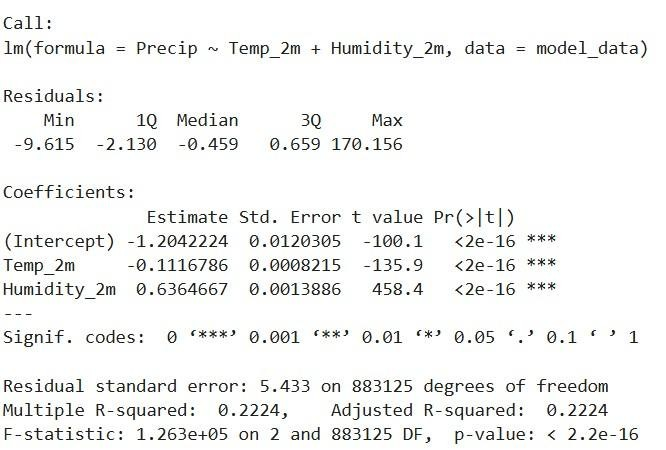
\includegraphics[width=0.6\textwidth]{figures/regression.jpg}
\caption{Model summary}
\end{figure}

\subsubsection*{Step 4: Model Evaluation}

To assess the model’s performance, we calculate:

\begin{itemize}
  \item \textbf{R-squared (R\(^2\))}: Measures how well the predictors explain the variance in the target variable. Values closer to 1 indicate a better fit.
  \item \textbf{Mean Squared Error (MSE)}: Measures the average squared difference between actual and predicted values. Lower MSE indicates better accuracy.
\end{itemize}

\begin{verbatim}
r_squared <- summary(model)$r.squared
mse <- mean((predictions - model_data$Precip)^2)

actual_avg <- mean(model_data$Precip)
predicted_avg <- mean(predictions)

cat("R-squared:", r_squared, "\n")
cat("Mean Squared Error (MSE):", mse, "\n")
cat("Actual Average Precipitation:", actual_avg, "\n")
cat("Predicted Average Precipitation:", predicted_avg, "\n")
\end{verbatim}

% Figure here-----------------------------
\begin{figure}[h]
\centering
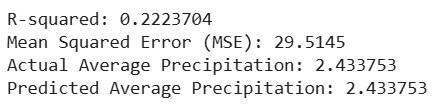
\includegraphics[width=0.5\textwidth]{figures/r_square.jpg}
\caption{Model evaluation metrics}
\end{figure}

\subsubsection*{Step 5: Visualizing Model Performance}

\textbf{Actual vs Predicted Plot:} This scatter plot compares the real precipitation values against the model’s predictions. The red line (y = x) indicates perfect prediction. Points close to this line show accurate predictions.

\begin{verbatim}
plot(model_data$Precip, predictions,
     xlab = "Actual Precipitation",
     ylab = "Predicted Precipitation",
     main = "Actual vs Predicted Precipitation")
abline(0, 1, col = "red")
\end{verbatim}

\textbf{Residual Plot:} This shows the residuals (errors) from the predictions. Ideally, residuals should be randomly scattered around zero. Patterns in residuals could suggest issues with the model fit.

\begin{verbatim}
residuals <- model$residuals
plot(residuals, main = "Residuals",
     ylab = "Residuals", xlab = "Index")
abline(h = 0, col = "red")
\end{verbatim}

% Figure here----------------------------
\begin{figure}[h]
\centering
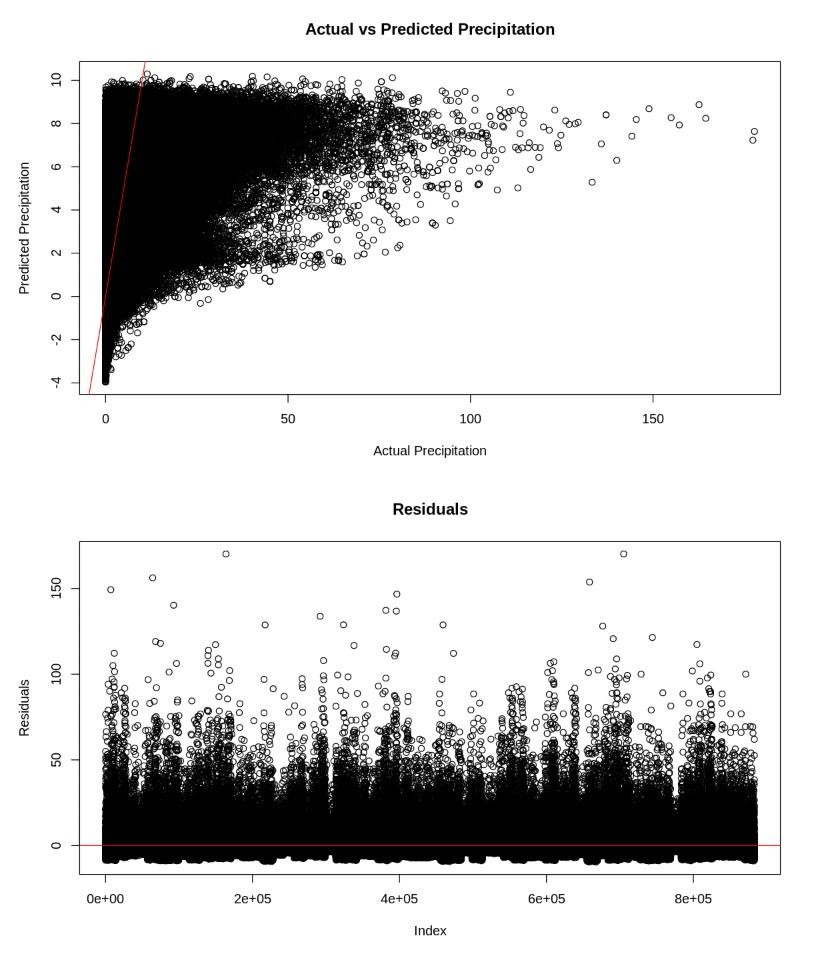
\includegraphics[width=0.5\textwidth]{figures/pred_residual.jpg}
\caption{Actual vs Predicted Plot and Residual Plot}
\end{figure}

\subsection*{Conclusion}

Through this exercise, we’ve seen how a simple regression model can be applied to climate data. We evaluated the model’s effectiveness using statistical metrics and visualizations, which are essential for interpreting the reliability and accuracy of predictions. As you explore more advanced models, this foundational approach will remain a critical tool for climate data analysis.
\clearpage

\subsection*{Predicting the Likelihood of Rainfall Based on Temperature and Humidity}

In this section, we’ll build a logistic regression model to predict whether rainfall will occur, using temperature and humidity as predictors. Instead of predicting how much rain will fall, we simplify the problem into a binary classification: Did it rain or not?

\subsubsection*{Step 1: Preparing the Data}

We start by creating a new variable in our dataset called \textit{Rain Occurrence}. This variable holds:

\begin{itemize}
  \item 1 if precipitation is greater than 0mm (indicating it rained)
  \item 0 otherwise (indicating no rain).
\end{itemize}

\begin{verbatim}
rain_data <- climate_data %>%
  mutate(Rain_Occurrence = ifelse(Precip > 0, 1, 0)) %>%
  select(Temp_2m, Humidity_2m, Rain_Occurrence)
\end{verbatim}

\subsubsection*{Step 2: Splitting the Dataset}

We divide our data into two parts:

\begin{itemize}
  \item \textbf{Training Set (80\%):} Used to train the model.
  \item \textbf{Testing Set (20\%):} Used to evaluate model performance.
\end{itemize}

\begin{verbatim}
set.seed(123)
train_index <- createDataPartition(rain_data$Rain_Occurrence, p = 0.8, 
list = FALSE)
train_data <- rain_data[train_index, ]
test_data <- rain_data[-train_index, ]
\end{verbatim}

\subsubsection*{Step 3: Standardizing the Features}

Before training, we standardize the temperature and humidity values to have a mean of 0 and a standard deviation of 1. This ensures that all features contribute equally to the model.

\begin{verbatim}
preprocess <- preProcess(train_data[, c("Temp_2m", "Humidity_2m")], 
method = c("center", "scale"))
train_data[, c("Temp_2m", "Humidity_2m")] <- predict(preprocess, 
train_data[, c("Temp_2m", "Humidity_2m")])
test_data[, c("Temp_2m", "Humidity_2m")] <- predict(preprocess, 
test_data[, c("Temp_2m", "Humidity_2m")])
\end{verbatim}

\subsubsection*{Step 4: Training the Logistic Regression Model}

We now fit a logistic regression model. This model estimates the probability of rain occurring based on the input temperature and humidity.

\begin{verbatim}
logistic_model <- glm(Rain_Occurrence ~ Temp_2m + Humidity_2m,
                      data = train_data, family = "binomial")
\end{verbatim}

\subsubsection*{Step 5: Making Predictions}

Once the model is trained, we make predictions on the test data:

\begin{itemize}
  \item Predicted Probability: the probability that rain will occur.
  \item Predicted Class: the classification (1 = rain, 0 = no rain) based on a threshold of 0.5.
\end{itemize}

\begin{verbatim}
test_data$Predicted_Prob <- predict(logistic_model, test_data,
type = "response")
test_data$Predicted_Class <- ifelse(test_data$Predicted_Prob > 0.5, 1, 0)
\end{verbatim}

\subsubsection*{Step 6: Evaluating the Model}

To assess the model’s effectiveness, we use a confusion matrix and compute several metrics:

\begin{itemize}
  \item \textbf{Accuracy:} Proportion of total correct predictions.
  \item \textbf{Precision:} Out of the times the model predicted rain, how often it was correct.
  \item \textbf{Recall (Sensitivity):} Out of the actual rainy instances, how many were correctly predicted.
  \item \textbf{F1-score:} Harmonic mean of precision and recall.
\end{itemize}

\begin{verbatim}
conf_matrix <- confusionMatrix(as.factor(test_data$Predicted_Class),
                               as.factor(test_data$Rain_Occurrence))

accuracy <- conf_matrix$overall["Accuracy"]
precision <- conf_matrix$byClass["Precision"]
recall <- conf_matrix$byClass["Recall"]
f1_score <- 2 * ((precision * recall) / (precision + recall))

cat("Accuracy:", accuracy, "\n")
cat("Precision:", precision, "\n")
cat("Recall:", recall, "\n")
cat("F1 Score:", f1_score, "\n")
\end{verbatim}

% Figure here----------------------------
\begin{figure}[h]
\centering
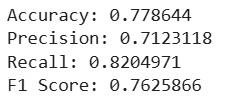
\includegraphics[width=0.3\textwidth]{figures/eval_metrics.jpg}
\caption{Evaluation metrics}
\end{figure}

\subsubsection*{Step 7: Visualizing Performance with the ROC Curve}

The ROC (Receiver Operating Characteristic) curve helps us visualize how well the model distinguishes between rainy and non-rainy days. The curve plots:

\begin{itemize}
  \item True Positive Rate (Recall) on the y-axis,
  \item False Positive Rate on the x-axis.
\end{itemize}

A curve closer to the top-left corner indicates better performance.

\begin{verbatim}
roc_curve <- roc(test_data$Rain_Occurrence, test_data$Predicted_Prob)
ggroc(roc_curve) +
labs(
  title = "ROC Curve", 
  x = "False Positive Rate", y = "True Positive Rate") +
theme_minimal()
\end{verbatim}

% Figure here--------------------------
\begin{figure}[h]
\centering
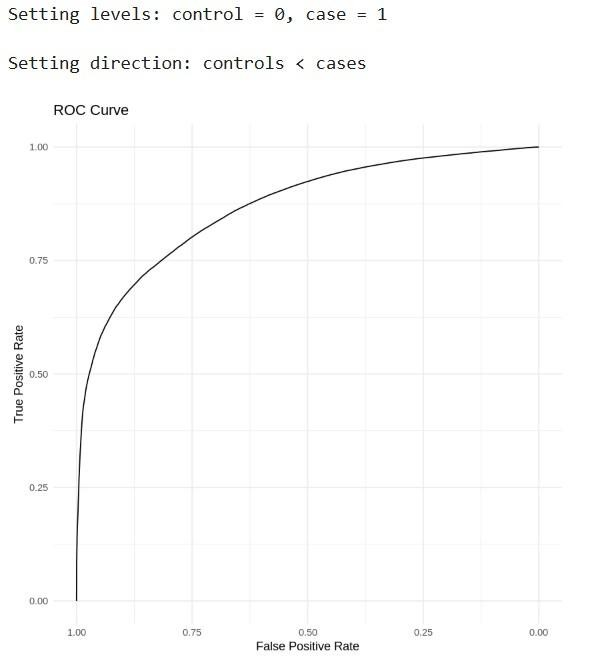
\includegraphics[width=0.5\textwidth]{figures/ROC.jpg}
\caption{ROC curve}
\end{figure}

\subsection*{Conclusion}

This logistic regression model gives us a practical tool to estimate the probability of rainfall using just temperature and humidity. While the model is simple, it introduces key classification concepts and serves as a foundation for more complex predictive techniques in climate analytics.

\section{Understanding Decision Trees}

A decision tree is one of the most intuitive and interpretable machine learning models used for both classification and regression tasks. In the context of climate analysis, decision trees help us understand how various atmospheric conditions contribute to an event such as heavy rainfall.


\subsection*{How Decision Trees Work}

A decision tree splits the dataset into branches based on the values of the input features. Each internal node represents a condition on a feature, and each leaf node represents an outcome.

The model continues to split the data into smaller groups to reduce uncertainty or “impurity.” In classification, a common measure for this impurity is the Gini Index or Entropy.

\begin{itemize}
  \item \textbf{Root Node:} The feature that best splits the data appears at the top.
  \item \textbf{Internal Nodes:} Represent decision rules based on features.
  \item \textbf{Leaf Nodes:} Represent class labels (e.g., 0 = No Heavy Rainfall, 1 = Heavy Rainfall).
\end{itemize}

\subsection*{Why Use Decision Trees in Climate Data?}

\begin{itemize}
  \item \textbf{Interpretability:} You can easily visualize and understand the rules that lead to predictions.
  \item \textbf{Non-linearity:} Trees can capture complex, non-linear interactions between variables.
  \item \textbf{No Need for Scaling:} Unlike many models, decision trees do not require feature standardization.
  \item \textbf{Handles Missing Values and Outliers:} Trees are robust to irregularities in the data.
\end{itemize}

\subsection*{Example Rule from the Tree}

Let’s say the decision tree discovers this rule: \\
If Humidity 2m $>$ 70 and Pressure $<$ 1010, then the model predicts Heavy Rainfall = 1.

This simple rule can help stakeholders quickly assess risk from available sensor readings.

\subsection*{Limitations of Decision Trees}

Despite their advantages, decision trees can overfit the training data if not carefully tuned. That means they may perform well on training data but poorly on unseen data. This can be mitigated by:

\begin{itemize}
  \item Pruning the tree (removing weak or unnecessary branches).
  \item Limiting the depth of the tree.
  \item Using ensemble methods (e.g., random forests or gradient boosting).
\end{itemize}

\subsection*{Visualizing the Tree Structure}

The tree diagram provides a clear representation of how the model splits the data and which features are most influential.

\begin{verbatim}
plot(tree_model)
text(tree_model, pretty = 0)
\end{verbatim}

This visualization not only shows the decision points but also helps explain the model’s logic to non-technical stakeholders, such as meteorologists or disaster management teams.

\subsection*{Classifying Heavy Rainfall Events Using Decision Trees}

To identify instances of heavy rainfall, we can use a decision tree model. In this section, we classify rainfall events as either Heavy or Not Heavy based on meteorological variables such as temperature, humidity, pressure, and wind speed.

We define a heavy rainfall event as one where precipitation exceeds the 75th percentile. The following R code demonstrates how to create and evaluate a decision tree model for this classification task.

\begin{verbatim}
# Install and load necessary package
install.packages("tree")
library(tree)
# Create a new column indicating heavy rainfall
precip_data <- climate_data %>%
  mutate(Heavy_Rainfall = ifelse(Precip > quantile(Precip, 0.75), 1, 0))
# Convert Heavy_Rainfall to factor for classification
precip_data$Heavy_Rainfall <- as.factor(precip_data$Heavy_Rainfall)
# Split data into training (80%) and testing (20%) sets
set.seed(123)
train_index <- createDataPartition(precip_data$Heavy_Rainfall, p = 0.8,
list = FALSE)
train_data <- precip_data[train_index, ]
test_data <- precip_data[-train_index, ]
# Train the decision tree model
tree_model <- tree(
Heavy_Rainfall ~ Temp_2m + Humidity_2m + Pressure + WindSpeed_10m, 
data = train_data)
# View summary of the model
summary(tree_model)
# Make predictions on test data
predictions <- predict(tree_model, test_data, type = "class")
# Evaluate the model using confusion matrix
conf_matrix <- table(Predicted = predictions, Actual = test_data$Heavy_Rainfall)
print(conf_matrix)
# Calculate performance metrics
accuracy <- sum(diag(conf_matrix)) / sum(conf_matrix)
precision <- conf_matrix[2, 2] / sum(conf_matrix[, 2])
recall <- conf_matrix[2, 2] / sum(conf_matrix[2, ])
f1_score <- 2 * (precision * recall) / (precision + recall)
# Print metrics
cat("Accuracy: ", accuracy, "\n")
cat("Precision: ", precision, "\n")
cat("Recall: ", recall, "\n")
cat("F1-score: ", f1_score, "\n")


\end{verbatim}

% Figure here---------------------------
\begin{figure}[h]
\centering
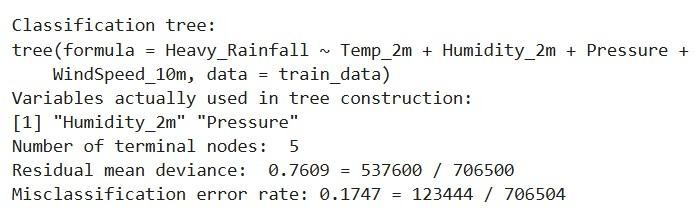
\includegraphics[width=0.5\textwidth]{figures/tree_summ.jpg}
\caption{Model summary}
\end{figure}

\begin{verbatim}
  # Visualize the decision tree
plot(tree_model)
text(tree_model, pretty = 0)
\end{verbatim}

% figure here----------------------------
\begin{figure}[h]
\centering
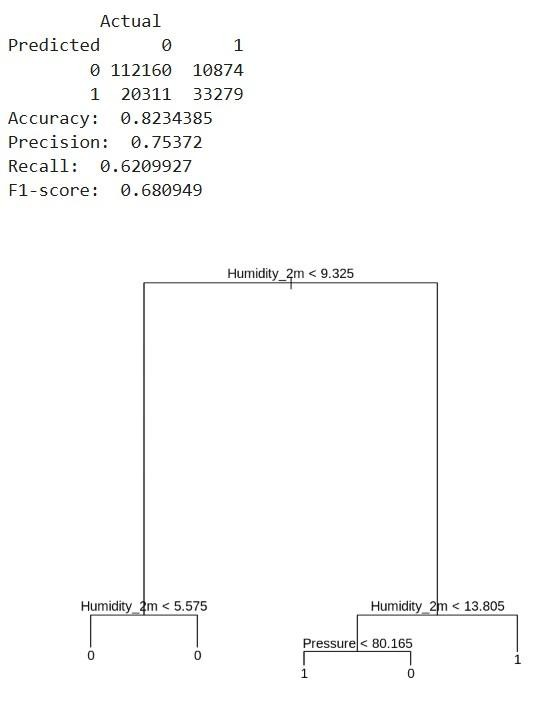
\includegraphics[width=0.5\textwidth]{figures/tree.jpg}
\caption{Classifying Heavy Rainfall Events Using Decision Trees}
\end{figure}

The decision tree model learns decision rules based on climate variables to classify whether a given observation is a heavy rainfall event.

The confusion matrix and the calculated performance metrics (accuracy, precision, recall, and F1-score) allow us to evaluate how well the model distinguishes between the two classes.

The visualization of the tree provides insight into which features most strongly influence the classification. This model can be improved or expanded by exploring ensemble techniques such as Random Forests or Gradient Boosting, which often provide more accurate and stable predictions.

\subsection*{Conclusion}

Decision trees offer a transparent and flexible way to classify rainfall events based on meteorological variables. When interpretability and ease of use are important, they can be an ideal choice in climate prediction applications.

\section{Cluster Analysis for Climatic Regions}

Cluster analysis is a powerful unsupervised machine learning technique used to identify natural groupings within data. In the context of climate science, cluster analysis helps uncover regions with similar climatic behavior, even when they may be geographically distant.

The idea is simple: group together climate observations that are more similar to each other than to those in other groups. This allows researchers and policymakers to:
\begin{itemize}
    \item Identify climate zones based on observed data (e.g., temperature, precipitation, humidity).
    \item Compare regional climate behaviors.
    \item Tailor climate adaptation strategies to similar zones.
\end{itemize}

\subsection*{How It Works}

Let’s say we have a dataset with climate measurements such as temperature, humidity, precipitation, and wind speed. Each row in our data represents a region or time-point, and our goal is to group these rows into “clusters” of similar climate patterns.

Key steps in the clustering process:
\begin{enumerate}
    \item \textbf{Feature Selection:} Choose the relevant variables (e.g., temperature, humidity).
    \item \textbf{Standardization:} Scale the variables so that each contributes equally to the clustering.
    \item \textbf{Choosing the Number of Clusters (K):} Decide how many climate groups to form using techniques like the elbow method.
    \item \textbf{Applying Clustering Algorithm:} Use algorithms like k-means to partition the data into K clusters.
    \item \textbf{Interpretation:} Analyze and visualize the clusters to understand regional patterns.
\end{enumerate}

\subsection*{Cluster Analysis for Climatic Patterns}

\textbf{Understanding the Goal}\\

Imagine you’re handed a huge table full of weather data with temperature, precipitation, humidity, and more from different regions or time periods. A natural question might arise: “Can we group these observations into meaningful climate categories?”

That’s where clustering helps. It automatically finds groups (called clusters) in your data that share similar features. Here, we want to find such clusters based on:
\begin{itemize}
    \item \texttt{Temp\_2m} – Temperature at 2 meters height
    \item \texttt{Precip} – Precipitation
\end{itemize}

\textbf{Step-by-Step Exploration}\\

\textbf{Step 1: Clean the Data} \\
Before we do any analysis, it’s important to make sure the data we’re using is complete. Missing values can interfere with calculations. So, we begin by removing any rows where \texttt{Temp\_2m} or \texttt{Precip} is missing.
\begin{verbatim}
climate_data_clean <- climate_data[complete.cases(climate_data$Temp_2m,
climate_data$Precip), ]
\end{verbatim}

\textbf{Step 2: Standardize the Data} \\
Temperature and precipitation are measured on different scales. Standardizing (scaling) makes sure each feature contributes equally to the clustering.
\begin{verbatim}
climate_scaled <- scale(climate_data_clean[, c("Temp_2m", "Precip")])
\end{verbatim}

\textbf{Step 3: Apply K-Means Clustering} \\
Now, we use a popular method called k-means clustering. We tell it to group the data into 3 clusters (this can be adjusted using the elbow method).
\begin{verbatim}
kmeans_result <- kmeans(climate_scaled, centers = 3, nstart = 10)
\end{verbatim}

Each observation is assigned a cluster number (1, 2, or 3), which we add back to the dataset:
\begin{verbatim}
climate_data_clean$Cluster <- as.factor(kmeans_result$cluster)
\end{verbatim}

\textbf{Step 4: Visualize the Clusters} \\
Let’s now “see” what those clusters look like. We plot temperature against precipitation, coloring each point by its cluster.
\begin{verbatim}
ggplot(climate_data_clean, aes(x = Temp_2m, y = Precip, color = Cluster)) +
  geom_point(size = 3) +
  labs(
    title = "Clustering of Climate Data (Temp_2m vs Precip)", 
       x = "Temperature (2m)", y = "Precipitation", color = "Cluster") +
  theme_minimal()
\end{verbatim}

\begin{figure}[h]
\centering
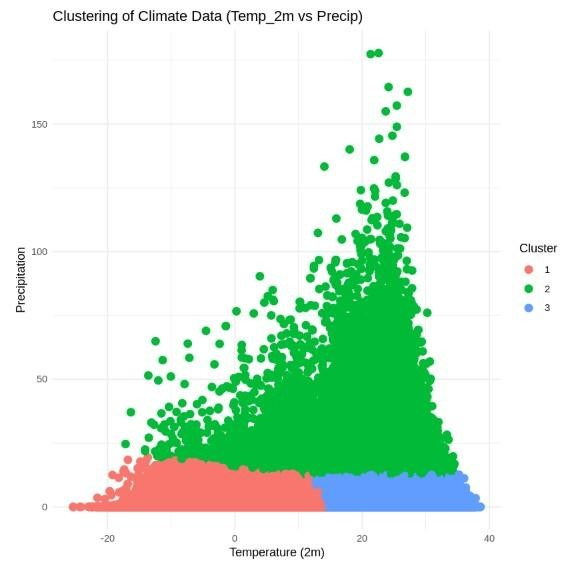
\includegraphics[width=0.5\textwidth]{figures/cluster.jpg}
\caption{Cluster Analysis for Climatic Patterns}
\end{figure}

Each color represents one cluster. The points in a cluster are close together, showing similar climate behavior.

\textbf{Why This Matters?}
\begin{itemize}
\item Clustering helps simplify large datasets into meaningful patterns. 
\item Each group can be analyzed separately to understand its unique climate profile. 
\item It’s useful for zoning, planning, and understanding environmental changes.
\end{itemize}

\textbf{Next Steps}\\

Now that we’ve performed basic clustering using k-means, we can explore:
\begin{itemize}
    \item Using more variables (e.g., humidity, pressure).
    \item Trying different clustering techniques (like hierarchical clustering).
    \item Mapping clusters onto geographical locations.
\end{itemize}

\section{ARIMA}

Time series forecasting is essential in many fields like finance, economics, climate science, and healthcare. One of the most widely used models for such forecasting is the ARIMA model, which stands for AutoRegressive Integrated Moving Average.

\subsection*{What is ARIMA?}

ARIMA combines three components:
\begin{itemize}
    \item \textbf{AR (AutoRegressive):} Uses past values to predict the current value.
    \item \textbf{I (Integrated):} Applies differencing to make the series stationary (removing trends).
    \item \textbf{MA (Moving Average):} Uses past forecast errors to predict current values.
\end{itemize}

The model is denoted as ARIMA(p, d, q):
\begin{itemize}
    \item \( p \): Number of autoregressive terms.
    \item \( d \): Number of times the data is differenced.
    \item \( q \): Number of lagged forecast errors.
\end{itemize}

\subsection*{Key R Libraries for ARIMA Modeling}

To apply ARIMA models in R, several useful packages are available that simplify the process of time series modeling and forecasting:
\begin{itemize}
    \item \textbf{stats} \\
    This is a base R package that provides the \texttt{arima()} function, which allows you to manually fit ARIMA models by specifying the values of \(p\), \(d\), and \(q\). It also includes the classic \texttt{ts()} function for creating time series objects.
    \begin{verbatim}
    fit <- arima(data, order = c(1,1,1))
    \end{verbatim}
    
    \item \textbf{forecast} \\
    Developed by Rob J Hyndman, this package provides the convenient \texttt{auto.arima()} function, which automatically selects the best ARIMA model based on AIC/BIC values. It also offers functions for forecasting, plotting, and evaluating models.
    \begin{verbatim}
    library(forecast)
    fit <- auto.arima(data)
    forecasted <- forecast(fit, h = 12)
    plot(forecasted)
    \end{verbatim}
    
    \item \textbf{tseries} \\
    This package supports time series analysis and includes the \texttt{adf.test()} for checking stationarity using the Augmented Dickey-Fuller test — a crucial step before fitting an ARIMA model.
    \begin{verbatim}
    library(tseries)
    adf.test(data)
    \end{verbatim}
    
    \item \textbf{ggplot2} \\
    While not specific to ARIMA, \texttt{ggplot2} is often used alongside these packages to create visually appealing time series plots and diagnostic graphs.
    \begin{verbatim}
    library(ggplot2)
    autoplot(forecasted)
    \end{verbatim}
\end{itemize}

These libraries together make it easy to preprocess, model, forecast, and visualize time series data in R using ARIMA.

\subsection*{ARIMA with R}

\textbf{Step 1: Data Aggregation}\\\\
We filtered the dataset for the district “Arghakhanchi,” extracted the year from the date, and computed the average temperature for each year.
\begin{verbatim}
temp_data <- climate_data %>% 
  filter(District == "Arghakhanchi") %>%
  mutate(Year = year(Date)) %>%  # Extract year from Date column
  group_by(Year) %>% 
  summarise(avg_temp = mean(Temp_2m, na.rm = TRUE)) %>%
  ungroup()
\end{verbatim}

Explanation of Parameters:
\begin{itemize}
    \item \texttt{Temp\_2m}: Daily temperature measured 2 meters above the ground.
    \item \texttt{na.rm = TRUE}: This argument removes any missing (NA) values during the computation of the mean, ensuring that incomplete data does not distort the result.
\end{itemize}

\textbf{Step 2: Time Series Conversion}\\\\ 
We converted the aggregated data into a time series object suitable for ARIMA modeling.
\begin{verbatim}
temp_ts <- ts(temp_data$avg_temp, 
start = min(temp_data$Year), frequency = 1) # Yearly data
\end{verbatim}

\textbf{Step 3: Fit ARIMA Model} \\ \\
We used the \texttt{auto.arima()} function, which automatically identifies the best ARIMA(p,d,q) model based on AICc (corrected Akaike Information Criterion).
\begin{verbatim}
model <- auto.arima(temp_ts)
summary(model)
\end{verbatim}

Explanation of Parameters:
\begin{itemize}
    \item \(p\): Autoregressive order — how many past values influence the present.
    \item \(d\): Differencing — how many times the data needs to be differenced to achieve stationarity.
    \item \(q\): Moving average order — how many past error terms influence the present.
\end{itemize}

\textbf{Step 4: Forecasting the Next 10 Years} \\ \\
We used the fitted model to forecast future average annual temperatures.
\begin{verbatim}
forecast_temp <- forecast(model, h = 10)
\end{verbatim}

Explanation of Parameters:
\begin{itemize}
    \item \(h = 10\): Forecast horizon — predicts for the next 10 time points (years).
\end{itemize}

\textbf{Step 5: Visualization of Forecast}\\ \\ 
We used \texttt{autoplot()} to visualize the forecast with confidence intervals.
\begin{verbatim}
autoplot(forecast_temp) + 
  ggtitle("10-Year Forecast of Average Annual Temperature\n(Arghakhanchi)") + 
  ylab("Average Temperature") + 
  xlab("Year")
\end{verbatim}

\begin{figure}[h]
\centering
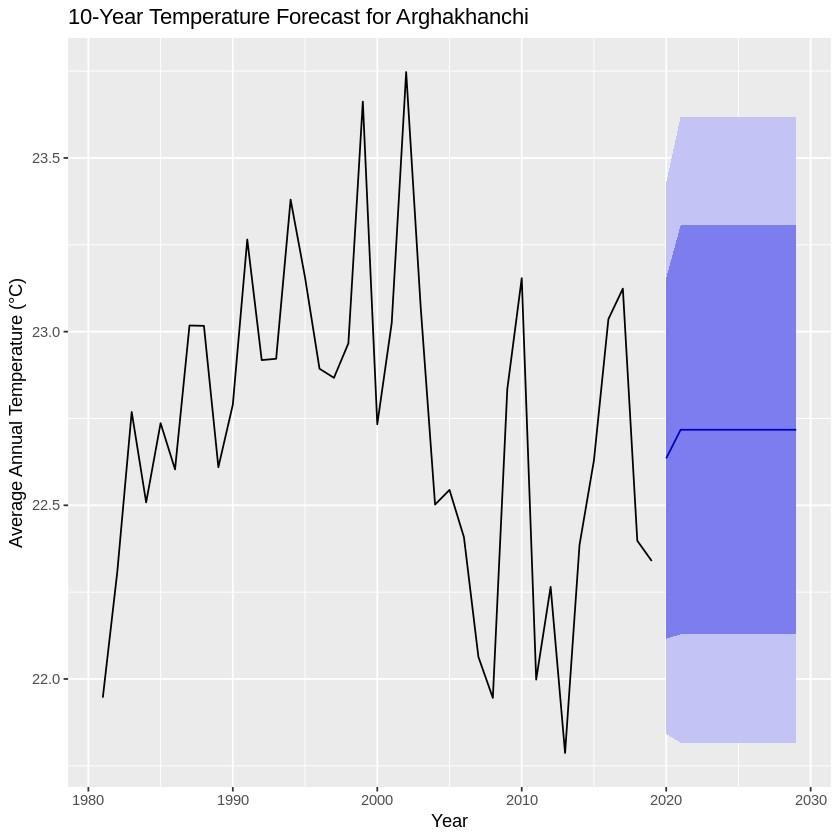
\includegraphics[width=0.5\textwidth]{figures/Arima.jpg}
\caption{10-Year Forecast of Average Annual Temperature in Arghakhanchi}
\end{figure}

\subsubsection*{Interpretation}
The shaded regions represent 80\% and 95\% confidence intervals. The solid line is the forecasted average temperature. The ARIMA model suggests expected trends based on past yearly averages and can guide climate planning or policy recommendations.
